 % This is the Reed College LaTeX thesis template. Most of the work
% for the document class was done by Sam Noble (SN), as well as this
% template. Later comments etc. by Ben Salzberg (BTS). Additional
% restructuring and APA support by Jess Youngberg (JY).
% Your comments and suggestions are more than welcome; please email
% them to cus@reed.edu
%
% See http://web.reed.edu/cis/help/latex.html for help. There are a
% great bunch of help pages there, with notes on
% getting started, bibtex, etc. Go there and read it if you're not
% already familiar with LaTeX.
%
% Any line that starts with a percent symbol is a comment.
% They won't show up in the document, and are useful for notes
% to yourself and explaining commands.
% Commenting also removes a line from the document;
% very handy for troubleshooting problems. -BTS

% As far as I know, this follows the requirements laid out in
% the 2002-2003 Senior Handbook. Ask a librarian to check the
% document before binding. -SN

%%
%% Preamble
%%
% \documentclass{<something>} must begin each LaTeX document
\documentclass[12pt,twoside]{reedthesis}
% Packages are extensions to the basic LaTeX functions. Whatever you
% want to typeset, there is probably a package out there for it.
% Chemistry (chemtex), screenplays, you name it.
% Check out CTAN to see: http://www.ctan.org/
%%
\usepackage{graphicx,latexsym}
\graphicspath{ {./figure/} }
\usepackage{amsmath}
\usepackage{amssymb,amsthm}
\usepackage{longtable,booktabs,setspace}
\usepackage{chemarr} %% Useful for one reaction arrow, useless if you're not a chem major
\usepackage[hyphens]{url}
% Added by CII
\usepackage{hyperref}
\usepackage{lmodern}
\usepackage{float}
\floatplacement{figure}{H}
% End of CII addition
\usepackage{rotating}


\usepackage{makeidx}
\makeindex


% Next line commented out by CII
%%% \usepackage{natbib}
% Comment out the natbib line above and uncomment the following two lines to use the new
% biblatex-chicago style, for Chicago A. Also make some changes at the end where the
% bibliography is included.
%\usepackage{biblatex-chicago}
%\bibliography{thesis}


% Added by CII (Thanks, Hadley!)
% Use ref for internal links
\renewcommand{\hyperref}[2][???]{\autoref{#1}}
\def\chapterautorefname{Chapter}
\def\sectionautorefname{Section}
\def\subsectionautorefname{Subsection}
% End of CII addition

% Added by CII
\usepackage{caption}
\captionsetup{width=5in}
% End of CII addition

% \usepackage{times} % other fonts are available like times, bookman, charter, palatino

% Syntax highlighting #22
  \usepackage{color}
  \usepackage{fancyvrb}
  \newcommand{\VerbBar}{|}
  \newcommand{\VERB}{\Verb[commandchars=\\\{\}]}
  \DefineVerbatimEnvironment{Highlighting}{Verbatim}{commandchars=\\\{\}}
  % Add ',fontsize=\small' for more characters per line
  \usepackage{framed}
  \definecolor{shadecolor}{RGB}{248,248,248}
  \newenvironment{Shaded}{\begin{snugshade}}{\end{snugshade}}
  \newcommand{\KeywordTok}[1]{\textcolor[rgb]{0.13,0.29,0.53}{\textbf{#1}}}
  \newcommand{\DataTypeTok}[1]{\textcolor[rgb]{0.13,0.29,0.53}{#1}}
  \newcommand{\DecValTok}[1]{\textcolor[rgb]{0.00,0.00,0.81}{#1}}
  \newcommand{\BaseNTok}[1]{\textcolor[rgb]{0.00,0.00,0.81}{#1}}
  \newcommand{\FloatTok}[1]{\textcolor[rgb]{0.00,0.00,0.81}{#1}}
  \newcommand{\ConstantTok}[1]{\textcolor[rgb]{0.00,0.00,0.00}{#1}}
  \newcommand{\CharTok}[1]{\textcolor[rgb]{0.31,0.60,0.02}{#1}}
  \newcommand{\SpecialCharTok}[1]{\textcolor[rgb]{0.00,0.00,0.00}{#1}}
  \newcommand{\StringTok}[1]{\textcolor[rgb]{0.31,0.60,0.02}{#1}}
  \newcommand{\VerbatimStringTok}[1]{\textcolor[rgb]{0.31,0.60,0.02}{#1}}
  \newcommand{\SpecialStringTok}[1]{\textcolor[rgb]{0.31,0.60,0.02}{#1}}
  \newcommand{\ImportTok}[1]{#1}
  \newcommand{\CommentTok}[1]{\textcolor[rgb]{0.56,0.35,0.01}{\textit{#1}}}
  \newcommand{\DocumentationTok}[1]{\textcolor[rgb]{0.56,0.35,0.01}{\textbf{\textit{#1}}}}
  \newcommand{\AnnotationTok}[1]{\textcolor[rgb]{0.56,0.35,0.01}{\textbf{\textit{#1}}}}
  \newcommand{\CommentVarTok}[1]{\textcolor[rgb]{0.56,0.35,0.01}{\textbf{\textit{#1}}}}
  \newcommand{\OtherTok}[1]{\textcolor[rgb]{0.56,0.35,0.01}{#1}}
  \newcommand{\FunctionTok}[1]{\textcolor[rgb]{0.00,0.00,0.00}{#1}}
  \newcommand{\VariableTok}[1]{\textcolor[rgb]{0.00,0.00,0.00}{#1}}
  \newcommand{\ControlFlowTok}[1]{\textcolor[rgb]{0.13,0.29,0.53}{\textbf{#1}}}
  \newcommand{\OperatorTok}[1]{\textcolor[rgb]{0.81,0.36,0.00}{\textbf{#1}}}
  \newcommand{\BuiltInTok}[1]{#1}
  \newcommand{\ExtensionTok}[1]{#1}
  \newcommand{\PreprocessorTok}[1]{\textcolor[rgb]{0.56,0.35,0.01}{\textit{#1}}}
  \newcommand{\AttributeTok}[1]{\textcolor[rgb]{0.77,0.63,0.00}{#1}}
  \newcommand{\RegionMarkerTok}[1]{#1}
  \newcommand{\InformationTok}[1]{\textcolor[rgb]{0.56,0.35,0.01}{\textbf{\textit{#1}}}}
  \newcommand{\WarningTok}[1]{\textcolor[rgb]{0.56,0.35,0.01}{\textbf{\textit{#1}}}}
  \newcommand{\AlertTok}[1]{\textcolor[rgb]{0.94,0.16,0.16}{#1}}
  \newcommand{\ErrorTok}[1]{\textcolor[rgb]{0.64,0.00,0.00}{\textbf{#1}}}
  \newcommand{\NormalTok}[1]{#1}

% To pass between YAML and LaTeX the dollar signs are added by CII
\title{Internship report}
\author{\textbf{Loïc Davadan}}
% The month and year that you submit your FINAL draft TO THE LIBRARY (May or December)
\date{21/05/2018 --- 20/08/2018}
\division{}
\advisor{\emph{Internship supervisor} : Thomas Goossens}
\supervisor{\emph{Institute supervisor} : Jean-Pierre Da Costa}
\institution{Centre de Recherches Agronomiques Wallon (CRA-W)}
\degree{}
\subtitle{AGROMET project : Investigating spatial interpolation of temperature
using Multiple Linear Regression}
\school{Bordeaux Sciences Agro}
\address{Rue de Liroux 9, 5030 Gembloux, Belgique}
%If you have two advisors for some reason, you can use the following
% Uncommented out by CII
% End of CII addition

%%% Remember to use the correct department!
\department{U11}
% if you're writing a thesis in an interdisciplinary major,
% uncomment the line below and change the text as appropriate.
% check the Senior Handbook if unsure.
%\thedivisionof{The Established Interdisciplinary Committee for}
% if you want the approval page to say "Approved for the Committee",
% uncomment the next line
%\approvedforthe{Committee}

% Added by CII
%%% Copied from knitr
%% maxwidth is the original width if it's less than linewidth
%% otherwise use linewidth (to make sure the graphics do not exceed the margin)
\makeatletter
\def\maxwidth{ %
  \ifdim\Gin@nat@width>\linewidth
    \linewidth
  \else
    \Gin@nat@width
  \fi
}
\makeatother

\renewcommand{\contentsname}{Table of Contents}
% End of CII addition

\setlength{\parskip}{0pt}

% Added by CII

\providecommand{\tightlist}{%
  \setlength{\itemsep}{0pt}\setlength{\parskip}{0pt}}

\Abstract{
The European directive 2009/128/CE imposes member-states to set up tools
that allow for a more rational use of crop protection products. The
AGROMET project, led by CRA-W, aims to generate a high spatial
resolution network which diffuses interpolated weather data provided by
physical weather stations using geostatistical tools. The internship
aimed to spatialize temperature using Multiple Linear Regression method.
To do that, the internship was integrated in in data acquisition and
data analysis steps. As a first step, data which can explain temperature
were collected and organised to integrate them in machine learning
algorithms. Then, the objective is to compare different combinations of
explanatory variables and to identify which one provides the lowest
error using multiple linear regression as learning method. The results
obtained from a database containing more than 23000 hours show some
interesting combinations as the one based on spatial coordinates and
elevation or the one based on the variables with the best linear
correlation computed every hour. Other variables will be integrated
afterward to try to reduce prediction errors.

~ ~

La directive européenne 2009/128/CE impose aux états-membres de mettre
en place des outils visant à une utilisation rationnelle des produits
phytosanitaires. Le projet AGROMET, dirigé par le CRA-W, a pour but de
genérer un réseau de stations virtuelles à haute résolution spatiale qui
diffusera des données météorologiques interpolées à partir de données
issues de stations physiques et d'outils géostatistiques. Le stage avait
pour objectif de spatialiser la température à l'aide de la Régression
Linéaire Multiple. Pour ce faire, le stage s'est intégré dans la phase
d'acquisition des données et d'analyse des données. Dans un premier
temps, des données qui pourraient expliquer la température ont été
récoltées et organisées afin de les intégrer dans des algorithmes de
machine learning. L'objectif est ensuite de comparer les différentes
combinaisons de variables explicatives et d'identifier celle qui fournit
les prédiction avec l'erreur la plus faible en utilisant la régression
linéaire multiple comme méthode d'apprentissage. Les résultats obtenus à
partir d'une base de données de plus de 23000 heures mettent en évidence
plusieurs combinaisons intéressantes comme celle utilisant les
coordonnées géographiques et l'altitude ou celle utilisant les variables
avec la meilleure corrélation linéaire à chaque heure. D'autres
variables seront par la suite intégrées pour tenter de réduire les
erreurs de prédiction.
}

\Abbreviations{
\begin{itemize}
\item
  API : Application Programming Interface
\item
  ANN : Artificial Neural Networks
\item
  CRA-W : Walloon agricultural research center
\item
  CRS : Coordinate Reference System
\item
  IDW : Inverse Distance Weight
\item
  JSON : JavaScript Object Notation
\item
  KNMI : Royal Netherlands Meteorological Institute (Dutch national
  weather service)
\item
  MAE : Mean Absolute Error
\item
  RMI : Royal Meteorological Institute
\item
  RMSE : Root Mean Square Error
\item
  OS : Operating System
\item
  SSH : Secure Shell
\item
  WGS84 : World Geodetic System 1984
\end{itemize}
}

\Definitions{
\begin{itemize}
\item
  to nest : \emph{imbriquer}
\item
  late blight : \emph{mildiou}
\item
  wheat septoria : \emph{septoriose du blé}
\item
  rain gauge : \emph{pluviomètre}
\item
  orange midge : \emph{cécidomyie orange du blé}
\item
  leaves wetness : \emph{humidité du feuillage}
\item
  forecast : \emph{prévision}
\end{itemize}
}


\Acknowledgements{
I would first like to thank my internship supervisor in the CRA-W Thomas
Goossens who accompanied and guided me throughout my intersnhip. He has
always been available to help me when I had questions or problems and he
has always put me back in the right direction.

I would like to thank the others members of the AGROMET project : the
project leader, Damien Rosillon, who trusted me throughout the
internship and Jean-Pierre Huart for his kindness and benevolence. I
also thank Viviane Planchon, the chief of the Unit 11 who trusted me for
the report about drought in Wallonia.

I also would like to thank the \emph{Youkou} team for its good mood and
kindness that made my internship even better.

I thank my school supervisor in \emph{Bordeaux Sciences Agro},
Jean-Pierre Da Costa, who accompanied me throughout my internship and
made sure my internship runs correctly.
}

\Dedication{

}

\Preface{
This document is my internship report for Bordeaux Sciences Agro as part
of my formation in ``Numérique pour l'Agriculture'' and my 3-month
internship in the CRA-W.

~

It was completely written with RMarkdown and \LaTeX.
}

% End of CII addition
%%
%% End Preamble
%%
%

\usepackage{amsthm}
\newtheorem{theorem}{Theorem}[chapter]
\newtheorem{lemma}{Lemma}[chapter]
\theoremstyle{definition}
\newtheorem{definition}{Definition}[chapter]
\newtheorem{corollary}{Corollary}[chapter]
\newtheorem{proposition}{Proposition}[chapter]
\theoremstyle{definition}
\newtheorem{example}{Example}[chapter]
\theoremstyle{definition}
\newtheorem{exercise}{Exercise}[chapter]
\theoremstyle{remark}
\newtheorem*{remark}{Remark}
\newtheorem*{solution}{Solution}
\begin{document}

% Everything below added by CII
  \maketitle

\frontmatter % this stuff will be roman-numbered
\pagestyle{empty} % this removes page numbers from the frontmatter
  \begin{acknowledgements}
    I would first like to thank my internship supervisor in the CRA-W Thomas
    Goossens who accompanied and guided me throughout my intersnhip. He has
    always been available to help me when I had questions or problems and he
    has always put me back in the right direction.
    
    I would like to thank the others members of the AGROMET project : the
    project leader, Damien Rosillon, who trusted me throughout the
    internship and Jean-Pierre Huart for his kindness and benevolence. I
    also thank Viviane Planchon, the chief of the Unit 11 who trusted me for
    the report about drought in Wallonia.
    
    I also would like to thank the \emph{Youkou} team for its good mood and
    kindness that made my internship even better.
    
    I thank my school supervisor in \emph{Bordeaux Sciences Agro},
    Jean-Pierre Da Costa, who accompanied me throughout my internship and
    made sure my internship runs correctly.
  \end{acknowledgements}
  \begin{preface}
    This document is my internship report for Bordeaux Sciences Agro as part
    of my formation in ``Numérique pour l'Agriculture'' and my 3-month
    internship in the CRA-W.
    
    ~
    
    It was completely written with RMarkdown and \LaTeX.
  \end{preface}
  \begin{abstract}
    The European directive 2009/128/CE imposes member-states to set up tools
    that allow for a more rational use of crop protection products. The
    AGROMET project, led by CRA-W, aims to generate a high spatial
    resolution network which diffuses interpolated weather data provided by
    physical weather stations using geostatistical tools. The internship
    aimed to spatialize temperature using Multiple Linear Regression method.
    To do that, the internship was integrated in in data acquisition and
    data analysis steps. As a first step, data which can explain temperature
    were collected and organised to integrate them in machine learning
    algorithms. Then, the objective is to compare different combinations of
    explanatory variables and to identify which one provides the lowest
    error using multiple linear regression as learning method. The results
    obtained from a database containing more than 23000 hours show some
    interesting combinations as the one based on spatial coordinates and
    elevation or the one based on the variables with the best linear
    correlation computed every hour. Other variables will be integrated
    afterward to try to reduce prediction errors.
    
    ~ ~
    
    La directive européenne 2009/128/CE impose aux états-membres de mettre
    en place des outils visant à une utilisation rationnelle des produits
    phytosanitaires. Le projet AGROMET, dirigé par le CRA-W, a pour but de
    genérer un réseau de stations virtuelles à haute résolution spatiale qui
    diffusera des données météorologiques interpolées à partir de données
    issues de stations physiques et d'outils géostatistiques. Le stage avait
    pour objectif de spatialiser la température à l'aide de la Régression
    Linéaire Multiple. Pour ce faire, le stage s'est intégré dans la phase
    d'acquisition des données et d'analyse des données. Dans un premier
    temps, des données qui pourraient expliquer la température ont été
    récoltées et organisées afin de les intégrer dans des algorithmes de
    machine learning. L'objectif est ensuite de comparer les différentes
    combinaisons de variables explicatives et d'identifier celle qui fournit
    les prédiction avec l'erreur la plus faible en utilisant la régression
    linéaire multiple comme méthode d'apprentissage. Les résultats obtenus à
    partir d'une base de données de plus de 23000 heures mettent en évidence
    plusieurs combinaisons intéressantes comme celle utilisant les
    coordonnées géographiques et l'altitude ou celle utilisant les variables
    avec la meilleure corrélation linéaire à chaque heure. D'autres
    variables seront par la suite intégrées pour tenter de réduire les
    erreurs de prédiction.
  \end{abstract}
  \begin{abbreviations}
    \begin{itemize}
    \item
      API : Application Programming Interface
    \item
      ANN : Artificial Neural Networks
    \item
      CRA-W : Walloon agricultural research center
    \item
      CRS : Coordinate Reference System
    \item
      IDW : Inverse Distance Weight
    \item
      JSON : JavaScript Object Notation
    \item
      KNMI : Royal Netherlands Meteorological Institute (Dutch national
      weather service)
    \item
      MAE : Mean Absolute Error
    \item
      RMI : Royal Meteorological Institute
    \item
      RMSE : Root Mean Square Error
    \item
      OS : Operating System
    \item
      SSH : Secure Shell
    \item
      WGS84 : World Geodetic System 1984
    \end{itemize}
  \end{abbreviations}
  \begin{definitions}
    \begin{itemize}
    \item
      to nest : \emph{imbriquer}
    \item
      late blight : \emph{mildiou}
    \item
      wheat septoria : \emph{septoriose du blé}
    \item
      rain gauge : \emph{pluviomètre}
    \item
      orange midge : \emph{cécidomyie orange du blé}
    \item
      leaves wetness : \emph{humidité du feuillage}
    \item
      forecast : \emph{prévision}
    \end{itemize}
  \end{definitions}
  \printindex

  \listoffigures

  \listoftables

  \hypersetup{linkcolor=black}
  \setcounter{tocdepth}{2}
  \tableofcontents

\mainmatter % here the regular arabic numbering starts
\pagestyle{fancyplain} % turns page numbering back on

\chapter*{Introduction}\label{introduction}
\addcontentsline{toc}{chapter}{Introduction}

Use of pesticides and other crop protection products is a topical issue
in an environmental and societal context. These products are
increasingly criticized for their risks and impacts on human health and
environment. Crop monitoring models are developed and their efficiency
is well demonstrated. Acting at the right time in plots is inscreasingly
possible thanks to these models. In Belgium, the Walloon agricultural
resarch centre (CRA-W) is a research centre where a lot of issues are
explored to bring solutions.

From May 22nd to August 20th, I did an internship in the (CRA-W). I
worked on the AGROMET project which is a project about agrometeorology
where the aim is to provide a near real-time hourly gridded datasets of
weather parameters at the resolution of 1 km² for the whole region of
Wallonia characterized by a quality indicator. This project is led by
the Farming Systems, Territory and Information Technologies Unit.

The internship has for objective to investigate a spatial interpolation
of the temperature using multiple linar regression with the best
combination of explanatory variables.

First, the report will present the CRA-W, its organisation, the Unit
where I worked and the project. Then, my workflow will be detailed in
two parts : the data acquisition and the data analysis through the
benchmark. Finally, the results will be interprated and discussed.

\chapter{Presentation of the AGROMET project and the
CRA-W}\label{presentation}

\section{CRA-W and Farming Systems, Territory and Information
Technologies
Unit}\label{cra-w-and-farming-systems-territory-and-information-technologies-unit}

The CRA-W was founded in 1872 and depends on the Regional Goverment of
Wallonia. It aims to maintain and develop the scientific excellence and
societal usefulness and contributes to sustainable development of the
agricultural industry in Wallonia in its economic, ecological and
cultural dimension. 120 scientifics are working in the CRA-W on three
sites (Gembloux, Libramont and Mussy-la-Ville) representing 300 ha of
fields, greenhouses, laboratories and offices. The CRA-W is a place for
scientific research but also to provide services in agricultural and
agri-food sector keeping a perspective view on the development of
agriculture.

~

The research is divided into 4 main fields where more than 100 projects
are currently in progress. :
\begin{itemize}
\tightlist
\item
  Precision agriculture
\item
  Precision livestock farming
\item
  Risk management
\item
  Understanding products
\end{itemize}
The CRA-W is divided into 4 departments with 4 research units each :
\begin{itemize}
\tightlist
\item
  Life sciences
\item
  Production et sectors
\item
  Valorisation of agricultural products
\item
  Agriculture and natural environment
\end{itemize}
~

The unit 11 \emph{Farming Systems, Territory and Information
Technologies} where I realized my internship belongs to the
\emph{Agriculture and natural environment} department. This Unit
develops tools to meet society's new expectations and decision support
systems to improve the technico-economic and environmental performance
of farming systems. There are actually 28 projects in progress.

The main activities of the Unit are the following :
\begin{itemize}
\tightlist
\item
  Adaptation of agrosystems to global change : definition of references
\item
  Adaptation of agrosystems to global change through bottom-up
  approaches
\item
  Support to the development of agrosystems in line with territory
  projects
\item
  Decision support systems and information technologies for the
  management of multifunctional agriculture
\item
  Spatial information systems for the management of rural areas.
\end{itemize}
~

PAMESEB is a non-profit organisation handled by the CRA-W which aims to
promote agrometeorology by considering weather conditions in the context
of walloon agriculture. PAMESEB manages a network of 30 automated
weather stations in Wallonia. These stations provide measures for ways
to fight crop diseases like late blight and wheat septoria. Stations
have a local acquisition unit for hourly data recording. The AGROMET
project uses weather data provided by the PAMESEB network as its primary
data source.

Each PAMESEB station is equipped with 5 basic sensors :
\begin{itemize}
\tightlist
\item
  Temperature sensor
\item
  Relative humidity sensor
\item
  Solar sensor
\item
  Wind sensor
\item
  Rain gauge
\end{itemize}
\section{The AGROMET project}\label{the-agromet-project}

\subsection{Context}\label{context}

The European directive 2009/128/CE imposes member-states to set up tools
that allow for a more rational use of crop protection products. Among
these tools, agricultural warning systems, based on crop monitoring
models for the control of pests and diseases are widely adopted and have
proved their efficiency. However, due to the difficulty to get
meteorological data at high spatial resolution (at the parcel scale),
they still are underused. The use of geostatistical tools (Kriging,
Multiple Regressions, ANN, etc.) makes it possible to interpolate data
provided by physical weather stations in such a way that a high spatial
resolution network (mesh size of 1 km2) of virtual weather stations
could be generated.

~

The purpose of the AGROMET project is to build a web platform that makes
such ``spatialized'' weather data available to crop monitoring models.
That will help other CRA-W's units and partners to act against crop
diseases like potato late blight or orange midge which depends on
meteorological conditions.

The project was inspired by several academic papers dealing with spatial
interpolation of data like \emph{Use of geographic information systems
in warning services for late blight} (Zeuner, 2007), \emph{Decision
Support Systems in Agriculture : Administration of Meteorological Data,
Use of Geographic Information Systems(GIS) and Validation Methods in
Crop Protection Warning Service} (Racca \emph{et al.}, 2011) and
\emph{Spatial interpolation of ambient ozone concentrations from sparse
monitoring points in Belgium} (Hooyberghs, 2006).

\subsection{Objectives}\label{objectives}

The project aims to set up an operational web-platform designed for
real-time agro-meteorological data dissemination at high spatial (1km2)
and temporal (hourly) resolution. To achieve the availability of data at
such a high spatial resolution, we plan to ``spatialize'' the real-time
data sent by more than 30 connected physical weather stations belonging
to the PAMESEB and RMI networks. This spatialization will then result in
a gridded dataset corresponding to a network of 17 000 virtual stations
uniformly spread on the whole territory of Wallonia.

These ``spatialized'' data will be made available through a web-platform
providing interactive visualization widgets (maps, charts, tables and
various indicators) and an API allowing their use on the fly, notably by
agricultural warning systems providers. An extensive and precise
documentation about data origin, geo-statistic algorithms used and
uncertainty will be also available.

~

The meteorological data the project aims to spatialize are :
\begin{itemize}
\tightlist
\item
  Temperature (1.5 meters above the ground)
\item
  Relative humidity (1.5 meters above the ground)
\item
  Leaves wetness
\item
  Rainfall will be spatialized from RMI rain radar data.
\end{itemize}
In order to perform spatial predictions of these variables, known
independent variables are required. Depending of the weather parameter
to be spatialized, various independent variables will be considered. We
can mention :
\begin{itemize}
\tightlist
\item
  Digital elevation model and its derivatives like aspect and slope
\item
  Solar irradiance
\item
  Other variables discussed to improve the prediction : distance to sea,
  CORINE land cover\ldots{}
\end{itemize}
The Figure \ref{fig:agromet} shows the global steps of the project and
steps before data diffusion.
\begin{figure}

{\centering 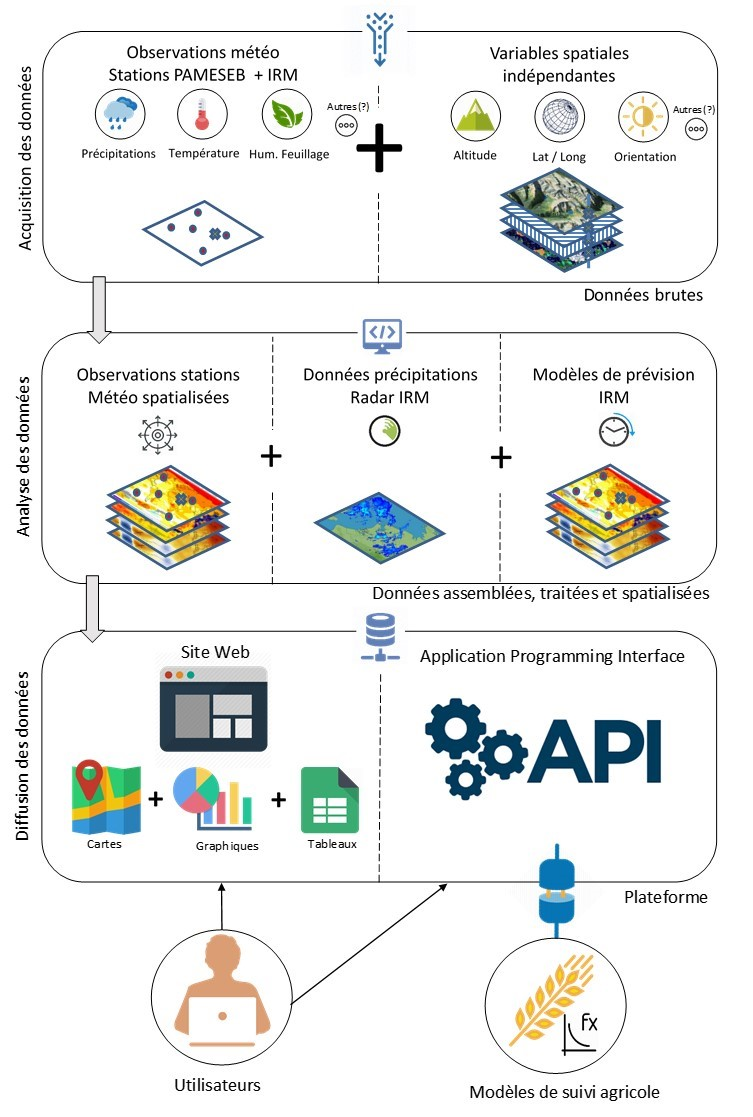
\includegraphics[width=0.65\linewidth]{figure/agromet} 

}

\caption{Global steps of the AGROMET project}\label{fig:agromet}
\end{figure}
\section{Scope of the internship : using multiple linear regression for
temperature
predictions}\label{scope-of-the-internship-using-multiple-linear-regression-for-temperature-predictions}

To perform spatial predictions of meteorological variables, several
statistical methods can be tested like multiple linear regression, ANN
and several kriging methods.

~

Two workpackages were clearly defined for my internship :
\begin{itemize}
\tightlist
\item
  acquiring and preparing independent variables that have been
  identified as potential explanatory variables for temperature
\item
  benchmarking various combinations of independent variables used with
  the \textbf{multiple linear regression} algorithm as spatial
  prediction method for the \textbf{temperature}
\end{itemize}
I used R because it is a free software for statistical computing and
graphics. Spatial data were collected from different sources and
involved the use of specific R libraries to manipulate them. I needed to
handle these libraries to manipulate vector and raster geodata. Then,
these data have been organised with the tidyverse library to respond to
the structure imposed by the chosen modeling library and to help reduce
computation time. The modeling library used is mlr, dealing with machine
learning algorithms, responds to a special architecture and logic that I
needed to understand. Then, the data have been integrated to build
models through a benchmark and analysis. Visualization was done thanks
to a plotting system for R, ggplot2, able to create graphics and maps.

The benchmark was run on two large years (from 2015-11-11 to 2018-06-30)
because some data were not available before this period.

\section{About the working
environment}\label{about-the-working-environment}

\subsection{Applications and tools}\label{applications-and-tools}

Working in development field often imposes to be methodic. In particular
for bug tracking or code versioning to detect errors and keep an history
of code modifications. Being methodic is also important for code
readability (adding comments for example) and code reproducibility. For
the reason that the AGROMET project is public, this last point is
important for transparency.

That's why preparing the working environment is important to help
achieve these good practices.

~

First, I have installed \textbf{Ubuntu GNOME}, a distribution of Linux
on my laptop. Indeed, this is an open-source OS prefered by developers.
It has a large community which is important to solve problems and bugs
and to improve the OS. Because it is free, anyone can install it and
that is important for reproducibility. Due to its large community of
developers, Linux is safer because they monitor for issues and can
repair them. Moreover, Linux has only 3\% of the market and hackers
prefer target a large segment of users as Windows. This installation of
Ubuntu was done thanks to a USB drive with a boot of Ubuntu GNOME.

~

Once I had Ubuntu installed on my laptop, I used an \textbf{ANSIBLE
script} to automatically install all the applications I need. Moreover,
this script handles the updates of these applications. That is a very
useful way to earn some time and it helps science reproductibility
because anyone with the script will end up with the exact same
installation.

~

Accessing to servers has to be secured to be protected against
intrusions and monitor logs. That's why every developer should have a
\textbf{SSH} key. This key or token is unique and enable people to
access to servers. It is useful to access to Git repositories for
example. It also helps to save some time because anyone who wants to
connect a service does not need to provide a login and password each
time using an SSH connection instead.

\textbf{GitHub} is a hosting service for version control. It facilitates
the collaborative work on a same code, the handle of code versions and
the use of code developed by other users. It is a very common tool for
developers because it ensures a public and online access.

For my internship, I had to collaboratively work on code development
with my mentor. This is why we have been using GitHub. For each of the
code folders that I had to work on, I made a fork that I've downloaded
on my laptop for further local developments. Then, I have a copy that I
can modify and I can send my modifications on GitHub. To clone these
repositories, my SSH key was useful.

~

The current development version of the AGROMET platform already offers
an \textbf{API} that allows to retrieve weather data from the stations.
A specific API token with reading rights has been created for my
internship. The API provides data in both JSON and GeoJSON formats which
are open-standard file formats. These formats are easy to parse by
machines and are easy to read by humans.

~

Among the different programming languages, R has been chosen because it
is is a free software environment for statistical computing and
graphics. It is adapted to data analysis because R was developed by
statisticians and easy to use even for people without programming
skills. R has a large community to help people to solve bugs and
problems and packages are well documented.

\textbf{Docker} is a software for containerizing platforms. This
container approach has many advantages compares to the use of virtual
machines : lightweight, quick and modular.

There are two main reasons to use R in conjunction with Docker. First,
it allows you to quickly and easily share your work whatever the OS and
R configuration of your collaborators. Second, it allows you to work in
an isolated environment. This means that you will never pollute your OS
and e.g.~run in time-consuming re-installation procedures due to broken
configuration. In case of OS crash, simply relaunch your Docker R
container with a single command and you are ready to work.

\subsection{Reproducible science}\label{reproducible-science}

Reproducible science refers to the idea that full working environment of
a research can be used by anyone to reproduce the results and create a
new work based on it. That ensures reliability and credibility because
the entire work is available.

~

In the case of the AGROMET project, the purpose of choosing open-source
is to allow reproducible science and transparency about the chosen
methods and therefore the meaning of the produced datasets.

Transparency is promoted thanks to open science. That means the content
and the results of the project will be accessible to others. Indeed,
transparency is superior to trust and is an ideal (Munafo, 2017).

Development represents the major part of the project. Today, open
science is widely used and tools have been developed for that. The
availability of code on GitHub ensures that anyone can check the code
and inspect it. Then, some people can improve codes and increase
efficiency of work.

Moreover, this transparency makes sure that people can inspect and
understand the origin of the data produced by the platforms. Users will
have a deep insight of the data they will be working with.

For these reasons, transparency and open science will give more
credibility and reliability to the project.

\chapter{Data acquisition and preparation}\label{data-acq}

Explanatory variables (i.e.~independent variables) are required to build
models able to predict the response variable (i.e.~dependent variable).
In our case the dependent variable is air temperature. We will call this
variable our \emph{target variable}. As set of explanatory variables
have been identified and integrated in our modeling approach. These will
be presented here below.

\section{Target variable}\label{target-variable}

The AGROMET project aims to provide weather data used as input for
various crop models. These parameters are temperature, relative
humidity, leaves wetness and rainfall. The last one is retrieved from
the RMI (Belgian Météo France equivalent). The others are measured by
weather stations from PAMESEB network, data are stored in a PostgreSQL
database and users can query it using the API. Using the API, users
retrieve untyped data and they have to type the data using specific
functions.

Temperature is the target variable concerned by my internship.

\section{Explanatory variables}\label{explanatory-variables}

As a reminder, the purpose of my internship was to implement the
multiple linear regression algorithm as a spatialization method. This
means that I need to find an equation where the target variable can be
modeled from one or more explanatory variables. The equation will have
the form : \(Y = b_0 + b_1.X_1 + b_2.X_2 + ... + b_n.X_n\) where \(Y\)
is the response variable and \(X_n\) your \(n\) explanatory variables
related to their estimated parameter \(b_n\).

These explanatory variables which have an influence on temperature are
already known and some academic papers already have dealt with them
(Zeuner 2007, Janssen 2011).

Two types of explanatory variables can be discriminated : static
variables, i.e.~variables not time-dependent but depending on the
spatial position and dynamic variables, i.e.~time-dependent and
position-dependent variables.

\subsection{Static variables}\label{static-variables}

\subsubsection{Land cover}\label{land-cover}

All PAMESEB weather stations are localized in agricultural or herbaceous
areas. That is a way to reduce errors about measures. However, the
surrounding environment (100 meters around the station) of each station
might be different and can have an impact on measures. For example, a
station could have a different behaviour if a forest is near its area or
if an artificial surface (road, construction) is near it.

CORINE land cover is an inventory updated every 6 years by
\textbf{Copernicus}, the European Union's Earth Observation Programme.
These data can also be found on the \textbf{Belgian geo-portal}. CORINE
Land Cover has been already used to make a spatial interpolation of air
pollution (Janssen \emph{et al.} 2011).

CORINE Land Cover is divided in 47 different land covers. 26 of them are
found in Wallonia. However, we made a clustering to group land covers
that we judge to have the same kind of impact on temperature. Then, we
made 5 classes :
\begin{itemize}
\item
  \textbf{Agricultural areas} : areas where crops can be tall
\item
  \textbf{Herbaceous vegetation} : cleared areas like pastures and
  grasslands
\item
  \textbf{Artificial areas} : roads, rails and constructions where
  anthropogenic material can impact temperature
\item
  \textbf{Forest} : large areas providing shadow and cold
\item
  \textbf{Water bodies} : areas like river, lake, wetlands and bogs.
  Finally, this class has been removed because of the fact that no
  stations are located near a water body
\end{itemize}
~

R can handle different two types of spatial data : vector and raster.
Vector model is based on points inside a CRS. Vector data can be points
or lines or polygons. In R, \texttt{sp} and \texttt{sf} packages can
handle this data type. The major difference between \texttt{sp} and
\texttt{sf} is that \texttt{sf} objects can be treated as data frames in
most operations and has better performances (Lovelace 2018). Raster
model is based on a matrix representing equally spaced pixels and
contains informations about the CRS, the extent and the origin.
\texttt{raster} package handles this data type. These three packages can
work together to convert data from a type to another one.

CORINE land cover data downloaded on the geo-portal was a shapefile,
i.e.~vector data, with WGS84 CRS. This geographic CRS has coordinates
expressed in degrees. Then, to read them in R, \texttt{sp} is necessary
but a conversion to \texttt{sf} was prefered for clustering for the
reasons given above.

A conversion of CRS was also done from WGS84 to Belgian Lambert 2008. In
contrast to WGS84, Lambert 2008 is a projected CRS expressed in meters.
It facilitates our work to characterize the surrounding environment of
the stations defining buffers around them. A projected CRS facilitates
the definition of the radius of the buffer using meters instead of
degrees.

~

Thanks to these buffers, part of each class of land cover is computed
and then stored in a table. These buffers have a radius of 100 meters
for physical stations and 500 meters for virtual stations (because each
station covers 1 km²). The Table \ref{tab:clcperc} below shows the
structure of the data frame where each station identified by an ID has
the percentage of cover for each class.
\begin{table}

\caption{\label{tab:clcperc}Distribution of land covers around physical stations}
\centering
\begin{tabular}[t]{rrrrr}
\toprule
\textbf{sid} & \textbf{crops} & \textbf{artificial} & \textbf{forest} & \textbf{herbaceous}\\
\midrule
1 & 63.85818 & 4.265755 & 0.00000 & 31.83038\\
4 & 64.11932 & 35.834990 & 0.00000 & 0.00000\\
7 & 75.28137 & 0.000000 & 0.00000 & 24.67295\\
9 & 99.95431 & 0.000000 & 0.00000 & 0.00000\\
10 & 69.91902 & 0.000000 & 30.03530 & 0.00000\\
13 & 89.50912 & 0.000000 & 10.44519 & 0.00000\\
\bottomrule
\end{tabular}
\end{table}
\subsubsection{Digital Terrain Model}\label{digital-terrain-model}

In the same way as land cover, the terrain characteristics could have an
impact on temperature of the environment. These variables have been
integrated in the models made by Zeuner \emph{et al.} (2007) and the
relevance has been demonstrated several times.

Elevation data have been recovered for Wallonia from \textbf{NASA's
SRTM} providing a high-resolution (90 meters) topographic data. Then,
slope, aspect and roughess of terrain have been calculated with spatial
libraries implemented in R.

\subsection{Dynamic Variables}\label{dynamic-variables}

\subsubsection{Solar irradiance}\label{solar-irradiance}

Some explanatory variables for temperature can be time-dependent. In
this case, we can be interested in solar irradiance. Indeed, solar
irradiance has an impact on weather changes (Dewitte \emph{et al.}
2004).

~

Data are recovered from \textbf{EUMETSAT}, the European Organisation for
the Exploitation of Meteorological Satellites. They are produced every
30 minutes and expressed in W/m². These data are aggregated in hourly
data and they are queried using the API of AGROMET.

There are 875 points distributed in Wallonia where records are
available, this is not sufficient in our case where the objective is to
provide predictions with a precision of 1 km². The handle of these
spatial data with R packages was necessary to spatialize the records. To
do that, the IDW spatial interpolation method was used.

These data are available from 2015-11-11. As a consequence, models built
before this date do not use solar irradiance as explanatory variable.
However, solar irradiance is an interesting explanatory variable, that's
why no model was built before this date for my internship.

In parallel with that, PAMESEB stations also measure solar irradiance.
But only 27 stations are useable. The measures from weather stations are
used to build models from physical stations whereas the EUMETSAT
measures will be used later for the spatialization on the spatial grid
of Wallonia.

\subsubsection{Temperature forecasts}\label{temperature-forecasts}

The AGROMET project is supported by RMI, the Belgian equivalent of Météo
France. As a partner, RMI will provide temperature forecasts based on
their own algorithms. It was planned to integrate these data as
explanatory variables but at the time of my internship these were not
yet available.

\section{Data preparation}\label{data-preparation}

Once all the data are available, an important task is to organize them
to perform modeling. This organisation needs to respond to a methodic
approach :
\begin{itemize}
\tightlist
\item
  help reduce computation time
\item
  respond to the structure imposed by the chosen modeling library
\end{itemize}
Our choice turned to the use of the \texttt{mlr} package because it
provides an interface for machine learning using a lot of statistical
methods. The objective of data preparation is to make our data
mlr-compliant because the package needs data with a specific structure.
In particular, I needed to organize data to have one line for each
station containing values for every explanatory variable. Moreover, this
organisation must be done for every hour.

The first step consists of grouping data. Static and dynamic variables
are grouped in a data frame. Then, to reduce time computation and to
prepare the integration of the data frame for the modeling, there is a
way to nest data frames with the library purrr. In this way, it is
possible to have one single row for each hour but every row contains
data frames inside. The Figure \ref{fig:nested} shows how it looks. This
nested data frame is a efficient way to manipulate many sub-tables at
once.
\begin{figure}

{\centering 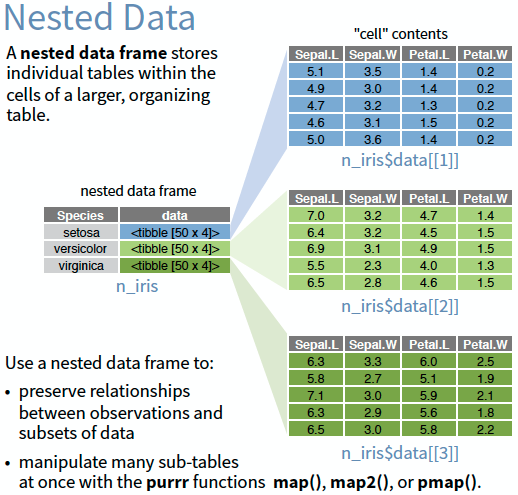
\includegraphics[width=0.5\linewidth]{figure/purrr_nest} 

}

\caption{Structure of a nested data frame}\label{fig:nested}
\end{figure}
In the case of the project, the nested data frame contains one row for
each hour which has a data frame containing data from each station at
this time. In the Table \ref{tab:ndf}, there is a preview of the data
frame contained into each row.
\begin{table}

\caption{\label{tab:ndf}Example of nested data frame in a row corresponding to 2016-05-19 15:00:00}
\centering
\resizebox{\linewidth}{!}{
\begin{tabular}[t]{r|r|r|r|r|r|r|r|r|r|r|r}
\hline
\textbf{altitude} & \textbf{slope} & \textbf{aspect} & \textbf{roughness} & \textbf{crops} & \textbf{artificial} & \textbf{forest} & \textbf{herbaceous} & \textbf{ens} & \textbf{tsa} & \textbf{X} & \textbf{Y}\\
\hline
473.6300 & 3.392046 & 211.6529 & 12.917668 & 63.85818 & 4.265755 & 0.00000 & 31.83038 & 348 & 12.4 & 721240.2 & 568849.6\\
\hline
345.7340 & 1.908891 & 162.7127 & 9.446796 & 64.11932 & 35.834990 & 0.00000 & 0.00000 & 389 & 12.8 & 714221.2 & 543453.8\\
\hline
348.8835 & 2.611751 & 165.0716 & 10.269126 & 75.28137 & 0.000000 & 0.00000 & 24.67295 & 779 & 14.1 & 750500.7 & 550825.6\\
\hline
497.7260 & 1.823958 & 137.0710 & 8.165029 & 99.95431 & 0.000000 & 0.00000 & 0.00000 & 916 & 13.5 & 753130.6 & 581716.9\\
\hline
389.9188 & 6.510637 & 310.6517 & 22.573696 & 69.91902 & 0.000000 & 30.03530 & 0.00000 & 916 & 14.9 & 734687.9 & 580969.6\\
\hline
259.7389 & 1.669001 & 288.5355 & 6.330072 & 89.50912 & 0.000000 & 10.44519 & 0.00000 & 774 & 15.2 & 641664.8 & 588814.6\\
\hline
\end{tabular}}
\end{table}
\chapter{Modeling with machine learning methods}\label{model}

Once the dataset is ready, the next step is to model spatial predictions
of temperature. To do that, machine learning is used through R.

\section{Principle of machine
learning}\label{principle-of-machine-learning}

\subsection{Definition}\label{definition}

Machine learning is the idea that there are generic algorithms that can
tell you something interesting about a set of data without you having to
write any custom code specific to the problem. Instead of writing code,
you feed data to the generic algorithm and it builds its own logic based
on the data. In other words, Machine learning is a subset of deep
learning or Artificial Intelligence that provides an ability to
``learn'' with data.

~

There are 2 types of machine learning : supervised and unsupervised
learning.

In practice, most of machine learning uses supervised learning.

~

From \emph{machinelearningmastery.com} :
\begin{quote}
Supervised learning is where you have input variables (x) and an output
variable (Y) and you use an algorithm to learn the mapping function from
the input to the output : Y = f(X).\\
The goal is to approximate the mapping function so well that when you
have new input data (x), you can predict the output variables (Y) for
that data.\\
It is called supervised learning because the process of an algorithm
learning from the training dataset can be thought of as a teacher
supervising the learning process
\end{quote}
~

For supervised machine learning, the algorithm tries to learn from
examples we give to it and then it returns a model of prediction.
Classification and regression are supervised machine learning.

This is the case of the AGROMET project where regression models are
used.

The unsupervised machine learning is not relevant in the context of my
work because this kind of machine learning does not need reference to
infer patterns and cannot be directly applied to regression problems.

\section{Machine learning approach in the AGROMET
project}\label{machine-learning-approach-in-the-agromet-project}

The objective is to spatially predict weather parameters (temperature,
relative humidity, leaves wetness). We use data from meteorological
stations and from other sources like EUMETSAT for solar irradiance and
COPERNICUS for land cover as explanatory variables for these weather
parameters and to build our models.

~

Here is our approach :

We choose a weather parameter to predict, it is our \textbf{target}. In
the context of my internship, \emph{temperature} is my target variable.

Then, from the historical dataset of hourly weather records from PAMESEB
database, a representative subset of records is filtered. Stations are
filtered to only keep the useful ones which are active. For each hourly
set of records, a benchmark experiment is run with multiple linear
regression algorithm, the \textbf{learner}, applied to various
regression \textbf{tasks}, i.e.~the target response variable
(temperature) and all the chosen \textbf{explanatory variables}
(elevation, slope, land cover\ldots{}). The different combinations of
explanatory variables using multiple linear regression algorithm are
compared and ranked using a \textbf{cross-validation resampling
strategy}. Several methods exist but we will use the Leave-One-Out
cross-validation method (LOOCV). It consists to establish, for each
hourly dataset, a model based on every weather stations except one which
will be the one where the model is tested to compute the error and then
doing it again as many times as the number of weather stations.
Performance metrics (RMSE and MAE) have been stored for each of these
iterations.

~

These performance metrics are two of the most common metrics used to
measure accuracy for continuous variables and for validation step in
machine learning.

~

MAE measures the average magnitude of the errors in a set of
predictions, without considering their direction. It is the average over
the test sample of the absolute differences between prediction and
actual observation where all individual differences have equal weight.

\[
MAE = \frac{1}{n} \sum_{i=1}^{n}{ \lvert y_{j} - \widehat{y}_{j} \rvert}
\]

~ ~

RMSE is a quadratic scoring rule that also measures the average
magnitude of the error. It is the square root of the average of squared
differences between prediction and actual observation.

\[
RMSE = \sqrt{\frac{1}{n} \sum_{i=1}^{n}{( y_{j} - \widehat{y}_{j} )^2}}
\]

The entire methodology is detailed in the \emph{Appendix A}
(Spatialization methodology).

\section{Machine Learning in R}\label{machine-learning-in-r}

All of our work is done using R. Moreover, a R package which provides
the infrastructure to run machine learning is available. This package
\textbf{mlr} is very complete to build models, make predictions and
evaluate performances.

Machine learning in R offers a common and simplified interface for all
statistical methods implemented in the package. With this package, run a
benchmark with several statistical methods can be done on data from a
period. This benchmark returns a lot of informations :
\begin{itemize}
\tightlist
\item
  about learners and task descriptions used in the benchmark
\item
  about models, test performance values, predictions from the benchmark
\end{itemize}
The package includes several ways to analyze benchmark results. Plots
are integrated to visualize results and learning algorithms can be
compared and ranked. It is possible to compare learners and tasks
through measures of error like RMSE or MAE. In the case ofmy internship,
the learner is always the same, multiple linear regression, and tasks
change because I modify the set of explanatory variables used.
\begin{figure}

{\centering 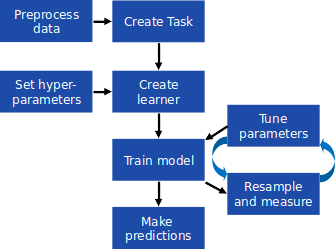
\includegraphics[width=0.5\linewidth]{figure/mlr_workflow} 

}

\caption{mlr workflow}\label{fig:mlr}
\end{figure}
The Figure \ref{fig:mlr} shows the general workflow of \texttt{mlr}.

~

This package has an important community which improves it regularly. A
lot of statistical methods are implemented from other packages like
\emph{tgp}, \emph{kknn} or \emph{DiceKriging}.

\chapter{Results and discussion}\label{results}

\section{Benchmark}\label{benchmark}

\subsection{Methodology}\label{methodology}

In the case of the project, a benchmark is an analysis where the
objective is to compare and rank the different combinations of tasks and
learners.

To realize this benchmark, data from 2015-11-11 00:00:00 to 2018-06-30
00:00:00 were used. The objective is to run a benchmark on 5 years of
data but at this moment, solar irradiance data from EUMETSAT were not
available before this date. Here, the dataset has 23089 hours.

~

The learners were defined with filter methods implemented in
\texttt{mlr}. These filter methods are applied to a statistical
algorithm (multiple linear regression) to choose explanatory variables
using conditions. The different conditions used to filter explanatory
variables are the following :
\begin{itemize}
\tightlist
\item
  for each hourly dataset, linear correlation with temperature is
  computed for every explanatory variable. Other filter methods are
  available (chi-squared, anova\ldots{}) but linear correlation seems to
  be the most relevant one for a regression problem.
\item
  then, explanatory variables are kept according to conditions :
  variables with the best hourly linear correlation with temperature
  (the number of variables to keep is specified) or all the variables
  which have a linear correlation greater than a value from 0 to 1.
\item
  I can also choose explanatory variables that I want to build models
  regardless of their linear correlation
\end{itemize}
All these filter methods where applied to \textbf{Multiple Linear
Regression} learner in the case of my internship.

~

The Table \ref{tab:explvar} shows the different combinations compared
using filter methods.

~

The benchmark performs for every hour and filter methods are applied
each time. As a consequence, linear correlation computation is hourly
done and \texttt{mlr} choose automatically the variables using the
filter methods. Then, based on this hourly computation, the combination
of explanatory variables can be different from one hour to another.

~

The benchmark took about 30 hours, i.e.~3 hours per method. Computations
are very long and results are very large. Each method represents more
than 1 Gigabyte of data.
\begin{table}

\caption{\label{tab:explvar}Combination of explanatory variables used}
\centering
\resizebox{\linewidth}{!}{
\begin{tabular}[t]{l|l|l}
\hline
\textbf{Statistical Method} & \textbf{ID} & \textbf{Explanatory variables}\\
\hline
Multiple Linear Regression & lm.Long.Lat & Longitude \& Latitude\\
\hline
Multiple Linear Regression & lm.Long.Lat.Elev & Longitude \& Latitude \& Elevation\\
\hline
Multiple Linear Regression & lm.SolIrr+1bestVar & Solar Irradiance \& best variable based on an hourly linear correlation computation\\
\hline
Multiple Linear Regression & lm.SolIrr+2bestsVar & Solar Irradiance \& 2 best variables based on an hourly linear correlation computation\\
\hline
Multiple Linear Regression & lm.SolIrr+3bestsVar & Solar Irradiance \& 3 best variables based on an hourly linear correlation computation\\
\hline
Multiple Linear Regression & lm.2bestsVar & 2 best variables based on linear correlation computation for every hour\\
\hline
Multiple Linear Regression & lm.3bestsVar & 3 best variables based on linear correlation computation for every hour\\
\hline
Multiple Linear Regression & lm.4bestsVar & 4 best variables based on linear correlation computation for every hour\\
\hline
Multiple Linear Regression & lm.Vars.r>0,5 & Variables with a linear correlation greater than 0.5\\
\hline
Multiple Linear Regression & lm.Vars.r>0,3 & Variables with a linear correlation greater than 0.3\\
\hline
\end{tabular}}
\end{table}
\subsection{Comparison of methods}\label{comparison-of-methods}

Once benchmark results are available, comparison of methods is possible.
This comparison is based on the error of measures. In our case, RMSE and
MAE were computed because they both express average model prediction
error in units of the variable of interest. Both metrics can range from
0 to \(\infty\) and are indifferent to the direction of errors. They are
negatively-oriented scores, which means lower values are better.

Since the errors are squared before they are averaged, the RMSE gives a
relatively high weight to large errors. This means the RMSE is more
useful because large errors are particularly undesirable in the project.
(Chai, 2014)

~

From the 10 methods compared, MAE and RMSE are computed and compared.
The results are shown in the Figure \ref{fig:meanerror}. In this case,
they both have the same behaviour. Indeed, they both return the same
ranking of the methods and they both show methods which stand out from
the other ones.

Multiple linear regression using coordinates to build models has a large
error, this combination is not relevant to spatially predict temperature
in Wallonia. Multiple linear regression using explanatory variables
whose their linear correlations with temperature is greater than 0.3 has
an error larger than the other methods too, this filter method is too
flexible to return valid spatial predictions. A few methods have a
similar error. In particular, that is the case when too many variables
are chosen to build models.

~

Among the three best methods, one is better than the others. This is the
models built from an equation using longitude, latitude and altitude as
explanatory variables. Tests realized on two months of data have already
shown that altitude is a powerful explanatory variable. The two other
methods are based on the hourly computation of the linear correlations
with temperature, with or without solar irradiance as mandatory variable
and keeping the 2 other best variables have a similar error. However, in
spite of their larger error, they can be interesting because the
equation is dynamic throughout hours and, in this way, the models are
adapted to the evaluated hour.
\begin{figure}

{\centering 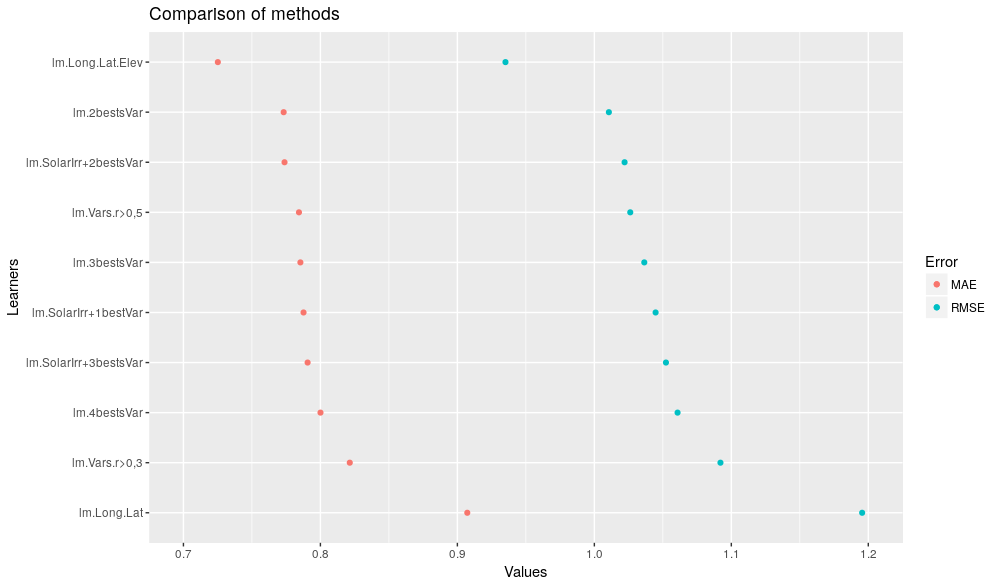
\includegraphics[width=1\linewidth]{figure/meanerror} 

}

\caption{Errors (RMSE and MAE) of methods}\label{fig:meanerror}
\end{figure}
Errors are between 0.72 and 0.91 for MAE and between 0.93 and 1.20 for
RMSE. These errors should be near zero. Both of MAE and RMSE are
expressed in degrees such as temperature. An error of 1 degree is
relatively important and has to be taken into consideration.

~

Performances of methods can be compared computing their rank for each
hour. The Figure \ref{fig:barchart} compares the three best methods :
\begin{itemize}
\tightlist
\item
  the 2 variables with the best hourly linear correlation with
  temperature
\item
  longitude, latitude and elevation
\item
  solar irradiance and the 2 variables with the hourly best linear
  correlation with temperature
\end{itemize}
This barchart corroborates the precedent graph. The method based on
coordinates and elevation is widely better than the two others which are
more similar but with a relevant difference. The ranks \(1.5\) and
\(2.5\) correspond to cases where two methods have exactly the same
error for a same task.
\begin{figure}

{\centering 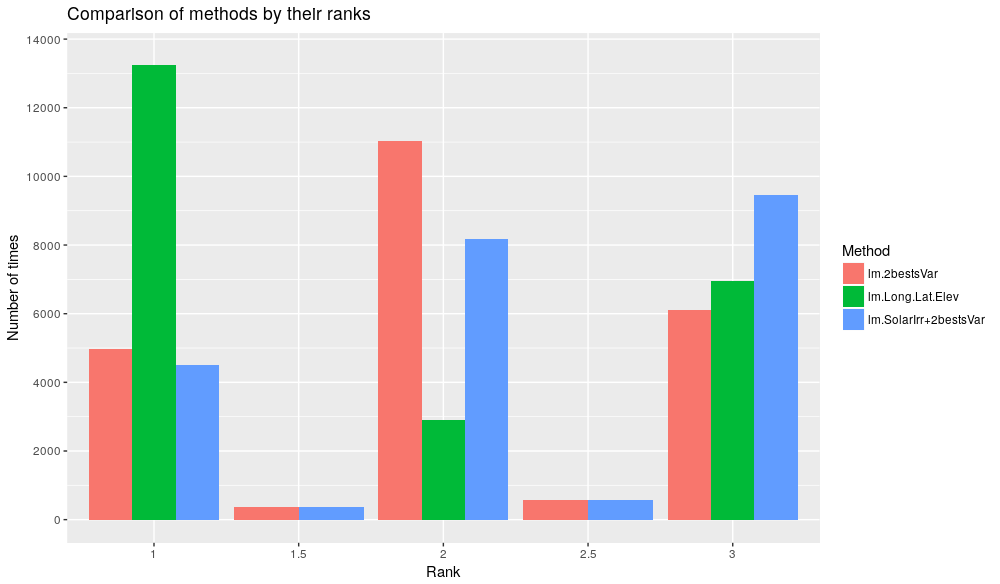
\includegraphics[width=1\linewidth]{figure/barchart} 

}

\caption{Comparison of methods by rank}\label{fig:barchart}
\end{figure}
For each hour, the equation of the model is computed. They can be
extracted from the benchmark. The Table \ref{tab:models} shows the
structure of the equations in the case where explanatory variables can
be different from one hour to another (lm.2bestsVar). The table also
shows what are the best variables and display the related error.
\begin{table}

\caption{\label{tab:models}Models with their equations}
\centering
\resizebox{\linewidth}{!}{
\begin{tabular}[t]{l|l|l|l|l|r|r}
\hline
\textbf{ } & \textbf{Datetime} & \textbf{Equation} & \textbf{BestVar1} & \textbf{BestVar2} & \textbf{RMSE} & \textbf{MAE}\\
\hline
16135 & 2017-09-13 06:00:00 & T = 14.656695 + -0.008887.altitude + 1e-06.X & altitude & X & 0.5674956 & 0.4107285\\
\hline
16136 & 2017-09-13 07:00:00 & T = 14.722147 + -0.00574.altitude + 0.012719.ens & altitude & ens & 0.6122121 & 0.4529545\\
\hline
16137 & 2017-09-13 08:00:00 & T = 15.676696 + -0.004304.altitude + -0.011732.herbaceous & altitude & herbaceous & 0.9375293 & 0.7287999\\
\hline
16138 & 2017-09-13 09:00:00 & T = 13.701668 + -0.012835.herbaceous + 0.00415.ens & herbaceous & ens & 1.2198397 & 0.9671947\\
\hline
16139 & 2017-09-13 10:00:00 & T = 14.987154 + -0.001473.altitude + -0.009431.herbaceous & altitude & herbaceous & 1.0206276 & 0.8224733\\
\hline
16140 & 2017-09-13 11:00:00 & T = 14.131936 + -0.003737.altitude + 0.005707.ens & altitude & ens & 0.8312792 & 0.5979420\\
\hline
16141 & 2017-09-13 12:00:00 & T = 11.852128 + -0.002653.altitude + 0.012421.ens & altitude & ens & 0.9727891 & 0.7488237\\
\hline
16142 & 2017-09-13 13:00:00 & T = 22.557946 + 0.003638.ens + -1.4e-05.Y & ens & Y & 1.2605875 & 0.9444467\\
\hline
16143 & 2017-09-13 14:00:00 & T = 15.441184 + 0.000484.altitude + -0.015099.herbaceous & altitude & herbaceous & 1.0796645 & 0.8760026\\
\hline
16144 & 2017-09-13 15:00:00 & T = 10.730857 + -0.003947.altitude + 9e-06.Y & altitude & Y & 0.9526830 & 0.7777128\\
\hline
\end{tabular}}
\end{table}
\subsection{Visualization}\label{visualization}

These models can be observed on maps. For that purpose, functions
building maps have been made with ggplot2 library from R for static maps
and leaflet library for interactive maps.

Models built from physical stations data are applied to the 1 km² grid
cells. Then, the temperature is mapped with a color palette similar to
the one of RMI. Class breaks are based on quantiles of temperature
values. Standard error is computed for each cell and it is shown on the
map with a white layer which has different levels of transparency
according to the error. A large standard error is related to an opacity
and vice-versa.

The Figure \ref{fig:map} shows an output for one hour based on the
method where explanatory variables are Solar irradiance and the 2
variables with the best linear correlation with temperature. To build
this map, some objects are needed : an object containing data
(temperature and standard error) for the grid and a spatial vector
object containing boundaries of Wallonia, but also the name of the
variable to display. Then, some conditions can be chosen, like the
display of the layer containing error, the display of the legend for
error, the way to build the legend and its classes. Some arguments
enable to customize the map with titles and comments. The function is
thus reusable for other usages. For example, the function builds maps
spatializing hydric deficit in Wallonia.

The choice I made was to use quantiles to make class breaks because that
is more relevant than homogeneous breaks.

The figure shows 2 maps. The one on the left is the map with
spatialization of temperature, the right one has the layer with error on
the temperature layer. It is possible to see regions where errors are
more important.
\begin{figure}
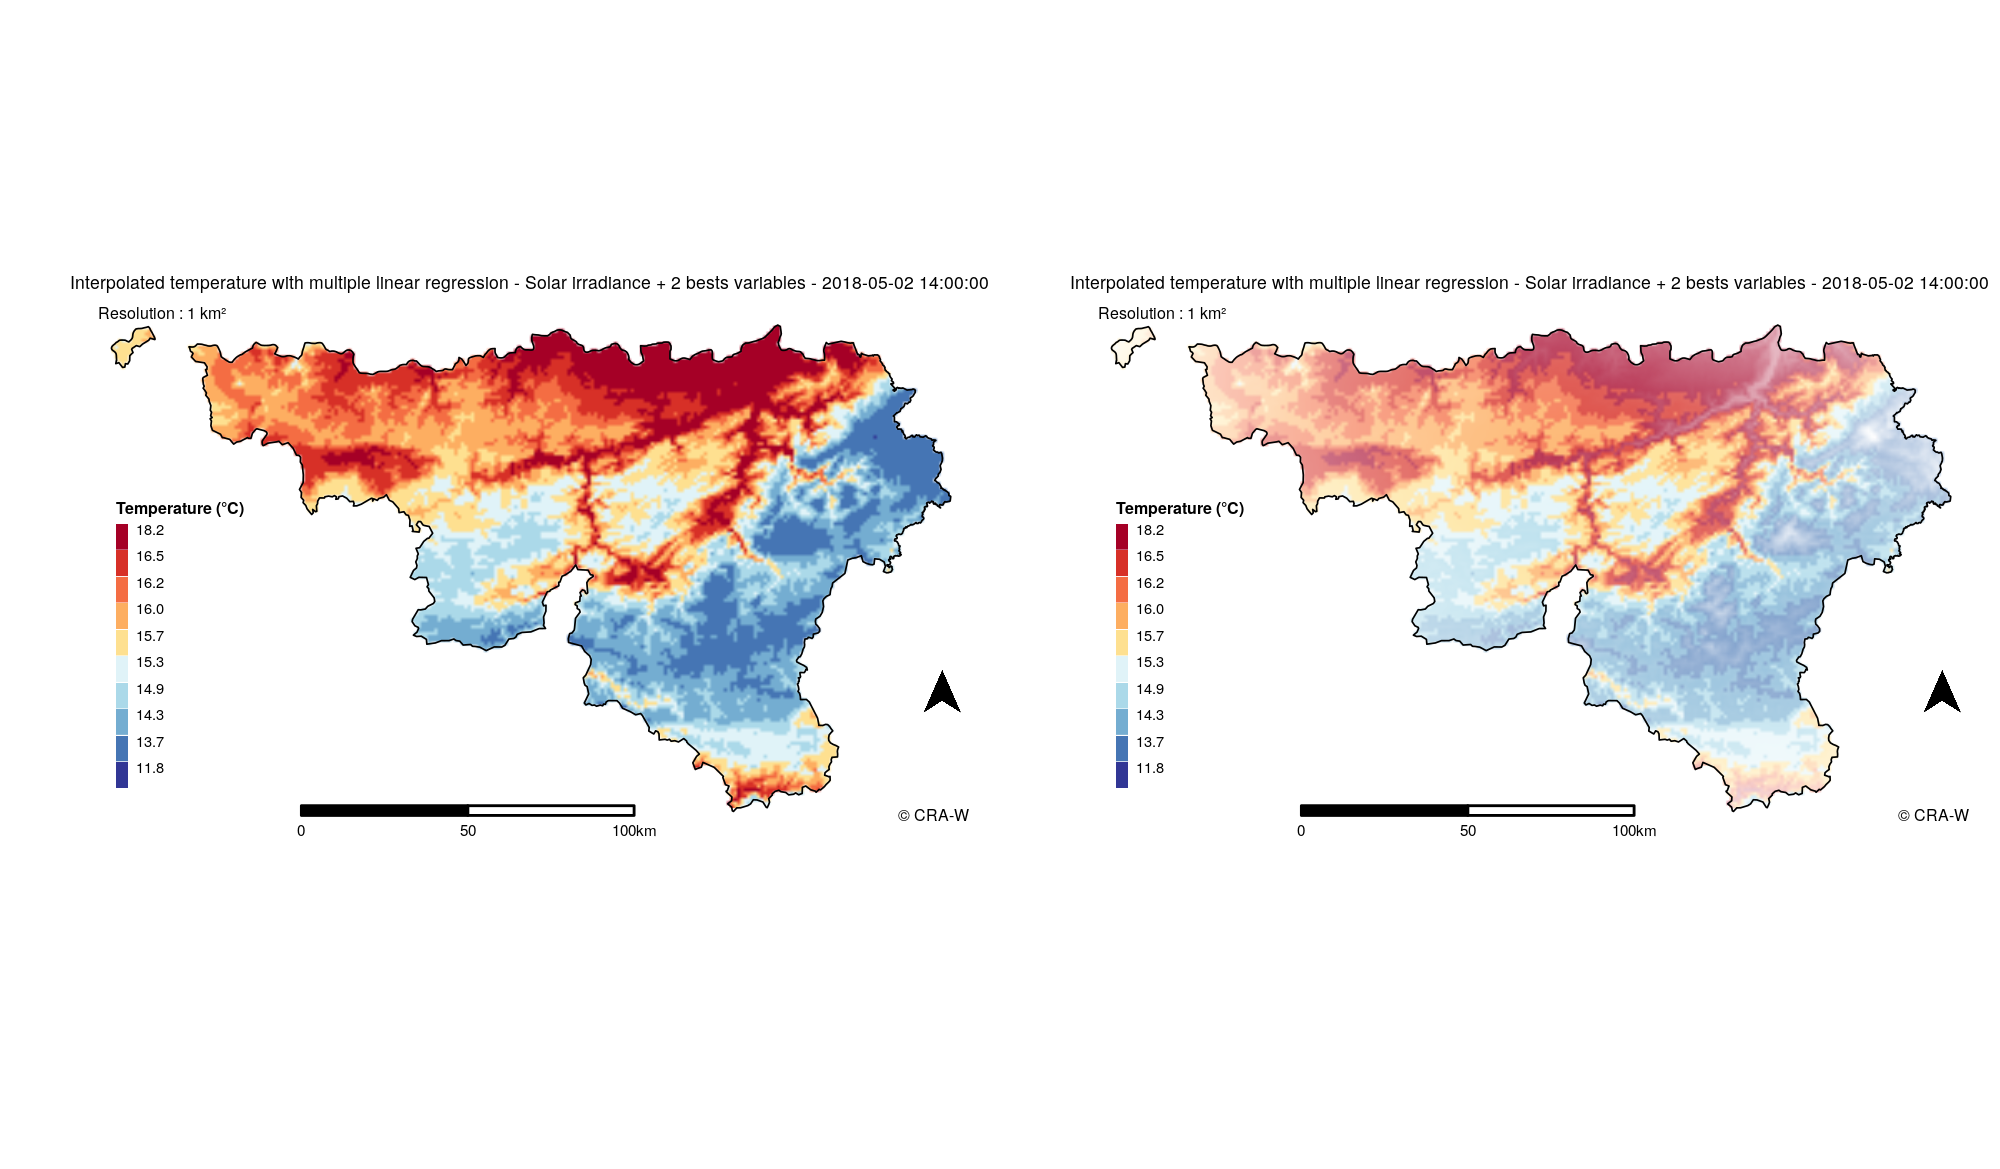
\includegraphics[width=1\linewidth]{figure/maperror} \caption{Example of an output for 2018-05-02 14:00:00 (left : without error ; right : with error)}\label{fig:map}
\end{figure}
This figure shows the output based on a model depending on the method
where explanatory variables are Solar irradiance and the 2 variables
with the best linear correlation with temperature, the equation of the
model is the following one :

\[
T = 15.59716 + -0.00629 \times Elevation + -0.00197 \times Herbaceous + 0.00206 \times SolarIrradiance
\]

These maps show whether the models are relevant. The \emph{Appendix B}
shows maps made with all methods for one hour. These maps show
differences in the relevance of each model. For example, the model
depending on longitude and latitude is very simplistic compared to the
others. The other models are more similar but show that some of them are
more reliable because the error is smaller. The better model is the
second one on the first row. It is corresponding to the the model
depending on longitude, latitude and elevation. For this hour, the
better model is the following : \[
T = -9.375042 + -0.010431 \times Elevation + 1.02e-05 \times Longitude + 1.59e-05 \times Latitude
\]

Longitude and latitude are expressed in meters because the CRS used is
Belgian Lambert 2008. That is why their coefficients are about
1\(e\)-05. For information, values of the coordinates are about
6\$e\$06.

\section{Discussion}\label{discussion}

As a reminder, the objective of the project is to provide weather
predictions. These predictions will feed decision support tools to
monitor crop diseases like potato late blight and to operate in fields
at the right times.
\begin{figure}

{\centering 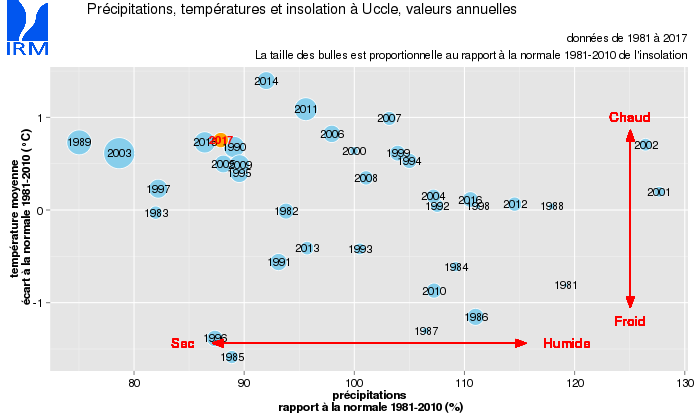
\includegraphics[width=400px,height=300px]{figure/rmi_climate_data} 

}

\caption{Precipitations, temperatures and insolation, annual values}\label{fig:rmi}
\end{figure}
Results have some limits that have to be discussed. The first limit is
the period used to build models. Indeed, models were built with data
from 2 and a half years. This period could be too short to be relevant.
Moreover, this period is not necessarily representative of a mean
period. According to RMI, 2015, 2017 and 2018 are hot and dry years
compared to normal year, 2016 were a wet year. This is shown on the
Figure \ref{fig:rmi}.

~

Even if visualization of outputs is not the main objective of the
project, the choice I made to compute class breaks with quantiles can be
discussed. In the case of temperature, that seems relevant but other
methods exist.

~

Models were built with some explanatory variables but they may be
insufficient. Adding new variables like temperature predictions from RMI
could improve models. Only 27 stations are used to build these models,
adding RMI stations network could be a solution to improve models too.
However, weather stations from different networks have differences in
their measures, checking interoperability is very important for that and
making corrections is essential.

~

Multiple linear regression is the only statistical method used to build
models, but going forward, other methods will be compared like ANN and
different kriging methods. The major constraint will be time computation
which is relatively long. There is a lot of possible combinations of
explanatory variables to compare, choices must be done because of the
time computation. These choices sometimes can be subjective and not
based on scientific literature.

~

Beyond these limits, other points can be discussed. Solar irradiance
data are provided by EUMETSAT and by PAMESEB stations. These data have
to be compared because both sources are used. Data from stations are
used to build models, data from EUMETSAT for spatialization. To do this
comparison, I have searched for the nearest point of record from
EUMETSAT to each PAMESEB station. Then, I compared each couple on the
period where I realised the benchmark. This comparison shows a
correlation around 0.95. As a consequence, there is nothing wrong with
it.

~

The ranking of the methods show that the method using the hourly 2 best
variables provides a smaller error than the same method adding solar
irradiance in every task. That is interesting because intuitively,
adding an explanatory variable should reduce the error. I noticed that
solar irradiance provides a large error for a few tasks, that might
explain these results.

~

With the aim to provide data for agronomic utilisation, there is an
interest to compare mean error observed in Wallonia and this error in
agricultural areas to be sure of the accuracy of predictions. That has
not be done yet.

~

Assuming that no other models will be better than those presented, there
will be a question of transparency for the project. In that way, models
will be clearly presented. If one static model is chosen for
predictions, this will be clear and transparent. But if the chosen
method is a dynamic one, using computation every hour, the method used
for each hour could be different, and that will have to be mentioned.

\chapter*{Conclusion}\label{conclusion}
\addcontentsline{toc}{chapter}{Conclusion}

At the end of this internship, the progress of the project is great.
Principal data have been recovered to be integrated as explanatory
variables and first models have been built. Now, the routine is ready to
build further models. First results are encouraging because models are
relatively relevant and they can be improved adding new explanatory
variables and using other statistical methods. Indeed, comparing models
with a lot of different methods will be possible to find the best
method, i.e.~the method with the smallest error (RMSE).

The project will end in 2020, that leaves time for building better
models and developing decision support tools for crop monitoring.
Therupon, the project will have an importance and some foreign
organisations are already interested by the project (Germany and
Slovenia).

Beyond the technical skills I developed during my internship, as the
utilisation of R language to interpolate spatial data and manipulating
them, the discovery of developer applications and tools like Docker or
Ubuntu, I also developed skills in collaborative work, in particular
with GitHub. It was a very enriching experience.

Outside the AGROMET project, I worked for other projects. I contributed
to the report on drought in this summer 2018 in Wallonia, upgrading
graphics and building a template of the map of Wallonia. I also
contributed to provide data from the API of the project to co-workers
for other projects.

\appendix

\chapter{Resources on AGROMET and my
work}\label{resources-on-agromet-and-my-work}
\begin{itemize}
\item
  European directive 2009/128/CE :
  \url{https://eur-lex.europa.eu/legal-content/EN/ALL/?uri=celex\%3A32009L0128}
\item
  PAMESEB network : \url{https://www.pameseb.be/}
\item
  Spatialization methodology available here :
  \url{https://pokyah.github.io/agrometeor-methodo-spatial/assets/uml_images/spatialization-methodology.svg}
\item
  All my codes are available on my Github account :
  \url{https://github.com/ldavadan}
\item
  My personal blog, made with Blogdown : \url{ldavadan.github.io}
\item
  Contribution to ``Crop and Grassland conditions in early August''
  report :
  \url{http://www.cra.wallonie.be/fr/etat-des-cultures-et-des-prairies-en-ce-debut-du-mois-daout-2018}
\end{itemize}
\chapter{Outputs with different
methods}\label{outputs-with-different-methods}

Methods from left to right and top to bottom follow the order presented
in Table \ref{tab:explvar}. Models built for 2018-03-07 14:00:00.
\begin{center}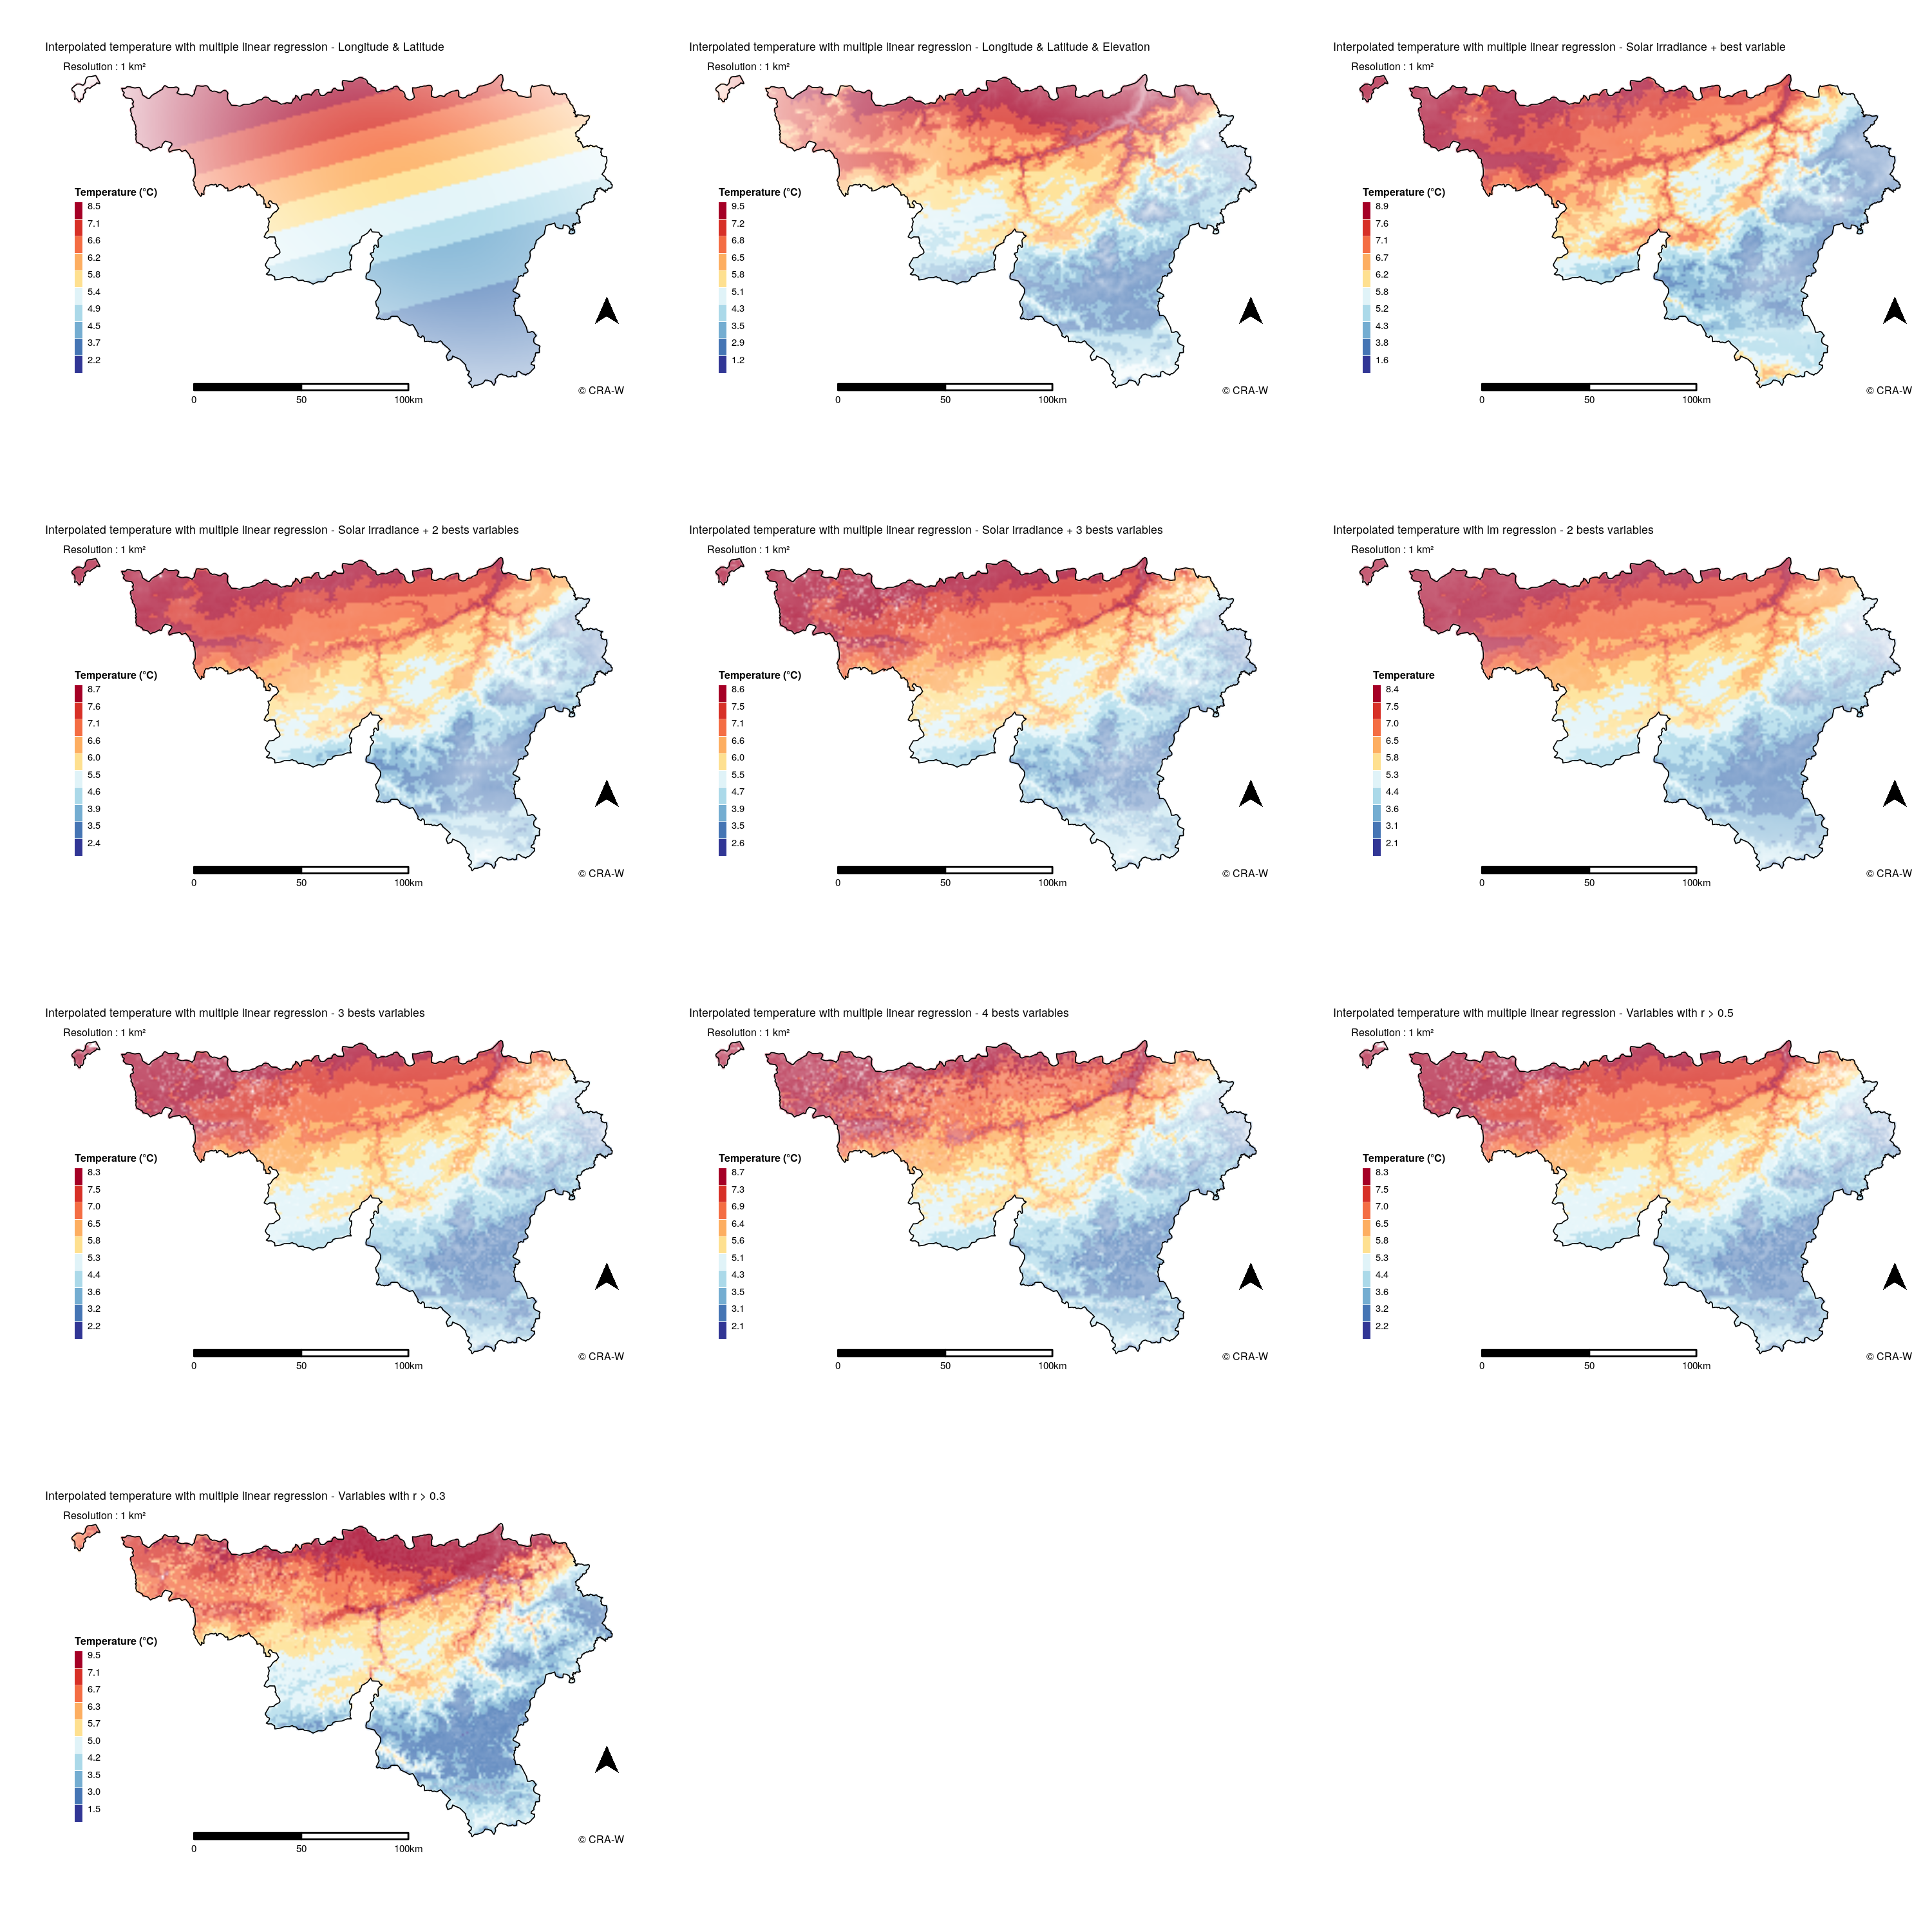
\includegraphics[width=1\linewidth]{figure/2018-03-07_14} \end{center}

\chapter{Additional resources}\label{additional-resources}
\begin{itemize}
\item
  Ubuntu GNOME : \url{https://ubuntugnome.org/}
\item
  ANSIBLE : \url{https://www.ansible.com/}
\item
  SSH : \url{https://www.ssh.com/}
\item
  GitHub : \url{https://github.com/}
\item
  API :
  \url{https://medium.freecodecamp.org/what-is-an-api-in-english-please-b880a3214a82}
\item
  R : \url{https://www.r-project.org/}
\item
  Docker : \url{https://www.docker.com/what-docker}
\item
  Copernicus :
  \url{https://land.copernicus.eu/pan-european/corine-land-cover/view}
\item
  Belgian Geoportal :
  \url{https://www.geo.be/\#!/catalog/details/bcd19aa9-c320-4116-971b-6e4376137f13?l=en}
\item
  NASA's SRTM : \url{https://lta.cr.usgs.gov/SRTM}
\item
  EUMETSAT :
  \url{https://landsaf.ipma.pt/en/products/longwave-shortwave-radiation/dssf/}
\item
  Machine Learning Mastery Blog :
  \url{https://machinelearningmastery.com/supervised-and-unsupervised-machine-learning-algorithms/}
\item
  Machine Learning in R : \url{http://mlr-org.github.io/mlr/index.html}
\end{itemize}
\chapter{Structure of the code using mlr
package}\label{structure-of-the-code-using-mlr-package}
\begin{Shaded}
\begin{Highlighting}[]
\CommentTok{# define learners}
\NormalTok{lrns.l <-}\StringTok{ }\KeywordTok{list}\NormalTok{(}\KeywordTok{makeFilterWrapper}\NormalTok{(}\DataTypeTok{learner =} \KeywordTok{makeLearner}\NormalTok{(}\DataTypeTok{cl =} \StringTok{"regr.lm"}\NormalTok{, }\DataTypeTok{id =} \StringTok{"lm.Long.Lat"}\NormalTok{), }\DataTypeTok{fw.method =} \StringTok{"linear.correlation"}\NormalTok{, }\DataTypeTok{fw.mandatory.feat =} \KeywordTok{c}\NormalTok{(}\StringTok{"X"}\NormalTok{, }\StringTok{"Y"}\NormalTok{), }\DataTypeTok{fw.abs =} \DecValTok{2}\NormalTok{),}
               \KeywordTok{makeFilterWrapper}\NormalTok{(}\DataTypeTok{learner =} \KeywordTok{makeLearner}\NormalTok{(}\DataTypeTok{cl =} \StringTok{"regr.lm"}\NormalTok{, }\DataTypeTok{id =} \StringTok{"lm.Long.Lat.Elev"}\NormalTok{), }\DataTypeTok{fw.method =} \StringTok{"linear.correlation"}\NormalTok{, }\DataTypeTok{fw.mandatory.feat =} \KeywordTok{c}\NormalTok{(}\StringTok{"X"}\NormalTok{, }\StringTok{"Y"}\NormalTok{, }\StringTok{"altitude"}\NormalTok{), }\DataTypeTok{fw.abs =} \DecValTok{3}\NormalTok{))}

\CommentTok{# define resampling strategy}
\NormalTok{resampling.l =}\StringTok{ }\KeywordTok{makeResampleDesc}\NormalTok{(}\DataTypeTok{method =} \StringTok{"LOO"}\NormalTok{)}

\CommentTok{#run benchmark}
\NormalTok{benchmark <-}\StringTok{ }\KeywordTok{benchmark}\NormalTok{(}
  \DataTypeTok{learners =}\NormalTok{ lrns.l[}\DecValTok{1}\NormalTok{],}
  \DataTypeTok{tasks =}\NormalTok{ data.stations.n.df}\OperatorTok{$}\NormalTok{tasks, }\CommentTok{# 1 task = 1 hour}
  \DataTypeTok{resamplings =}\NormalTok{ resampling.l,}
  \CommentTok{# additionnal parameters}
  \DataTypeTok{keep.pred =} \OtherTok{FALSE}\NormalTok{, }\CommentTok{# boolean specifying if predictions have to be kept}
  \DataTypeTok{show.info =} \OtherTok{TRUE}\NormalTok{, }\CommentTok{# boolean specifying if informations have to be shown when running}
  \DataTypeTok{models =} \OtherTok{FALSE}\NormalTok{, }\CommentTok{# boolean specifying if models have to be kept}
  \DataTypeTok{measures =} \KeywordTok{list}\NormalTok{(rmse, mae, timetrain) }\CommentTok{# list of measures to do}
\NormalTok{)}
\end{Highlighting}
\end{Shaded}
\backmatter

\chapter*{References}\label{references}
\addcontentsline{toc}{chapter}{References}

\markboth{References}{References}

\noindent

\setlength{\parindent}{-0.20in} \setlength{\leftskip}{0.20in}
\setlength{\parskip}{8pt}

\hypertarget{refs}{}
\hypertarget{ref-chai2014}{}
Chai, T., \& Draxler, R. (2014). Root mean square error (rmse) or mean
absolute error (mae)? -- Arguments against avoiding rmse in the
literature. \emph{Geoscientific Model Development}, 1247--1250.

\hypertarget{ref-dewitte2004}{}
Dewitte, S., \& others. (2004). Measurement and uncertainty of the
long-term total solar irradiance trend. \emph{Solar Physics}, 209--216.

\hypertarget{ref-hooyberghs2006}{}
Hooyberghs, J., \& others. (2006). Spatial interpolation of ambient
ozone concentrations from sparse monitoring points in belgium. \emph{J.
Environ. Monit.}, 1129--1135.

\hypertarget{ref-janssen2008}{}
Janssen, S., \& others. (2008). Spatial interpolation of air pollution
measurements using corine land cover data. \emph{Atmospheric
Environment, Volume 42, Issue 20}, 4884--4903.

\hypertarget{ref-munafo2017}{}
Munafo, M., \& others. (2017). A manifesto for reproducible science.
\emph{Nature Human Behaviour Volume 1, Article Number: 0021}.

\hypertarget{ref-racca2011}{}
Racca, P., \& others. (2011). Decision support systems in agriculture :
Administration of meteorological data, use of geographic information
systems (gis) and validation methods in crop protection warning service.
\emph{Efficient Decision Support Systems - Practice and Challenges from
Current to Future}, 331--354.

\hypertarget{ref-zeuner2007}{}
Zeuner, T., \& Kleinhenz, B. (2007). Use of geographic information
systems in warning services for late blight. \emph{Bulletin OEPP/EPPO},
327--334.

% Index?

\end{document}
